\section{Introduction}
\label{sec:intro}

Reinforcement learning (RL) has achieved impressive results in high-dimensional control, yet its application to real-world continuous navigation remains fundamentally limited. Modern deep RL methods such as SAC~\citep{haarnoja2018sac} and PPO~\citep{schulman2017ppo} typically require millions of interactions to learn a single robust policy, and their performance degrades sharply under even mild distribution shift. These challenges are amplified in simultaneous navigation and mapping (SNAM), where the agent must traverse unknown environments while building and updating spatial representations online. In this setting, long-horizon reasoning, multi-scale decision making, and the need for safe, sample-efficient adaptation often overwhelm existing methods.

\paragraph{Why many RL fails at SNAM.}
Three structural limitations are particularly acute in navigation:
(i) \emph{Sample efficiency}: continuous control demands rich exploration and fine-grained motor control; model-free RL compensates with massive data collection and unstable credit assignment.
(ii) \emph{Generalization}: black-box policies memorize training environments instead of discovering transferable navigation principles, leading to brittle behavior under new obstacle layouts or sensing conditions.
(iii) \emph{Temporal scale separation}: navigation couples fast obstacle avoidance, mid-range local planning, and slow global goal pursuit. Hierarchical RL~\citep{sutton1998between,vezhnevets2017feudal} introduces additional levels but still relies on monolithic value-based objectives and carefully engineered reward decompositions.

\begin{figure*}[htbp]
\centering
\setlength{\tabcolsep}{2pt}
\small\sffamily

\begin{tabular}{@{}c ccc@{}}
  & \textbf{Timestep A} & \textbf{Timestep B} & \textbf{Timestep C} \\[4pt]
  
  \rotatebox{90}{\parbox{20mm}{\centering\textcolor{red!65!black}{\textbf{Baseline}}}} &
  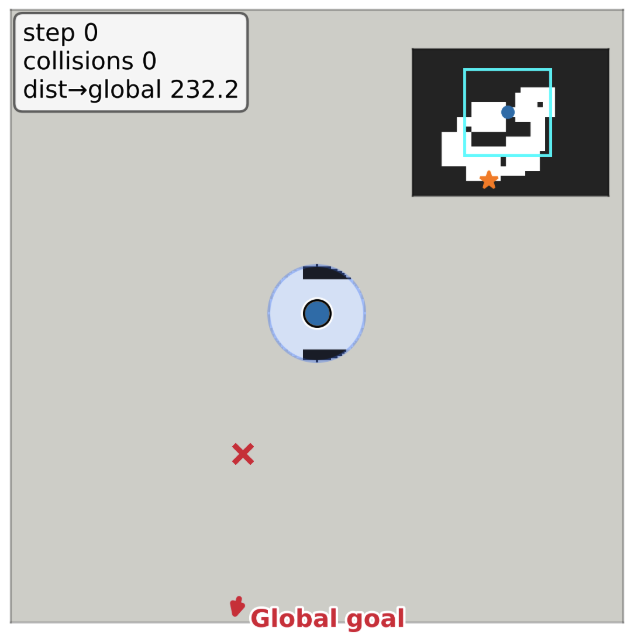
\includegraphics[width=0.29\linewidth]{baseline_A.png} &
  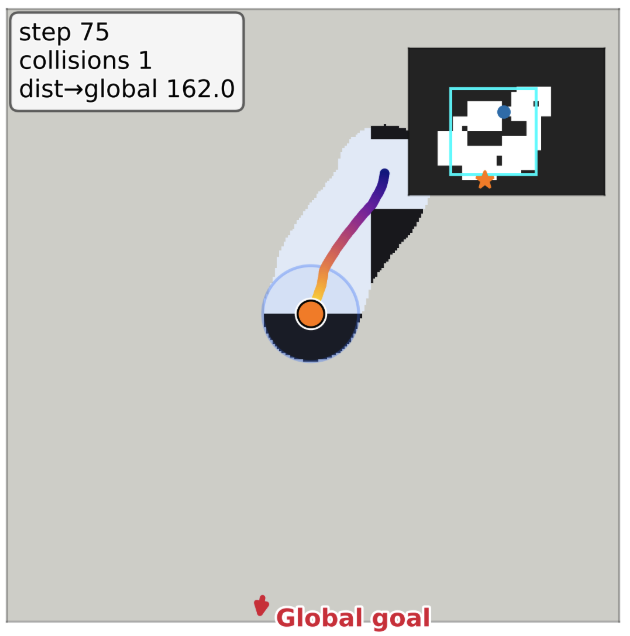
\includegraphics[width=0.29\linewidth]{baseline_B.png} &
  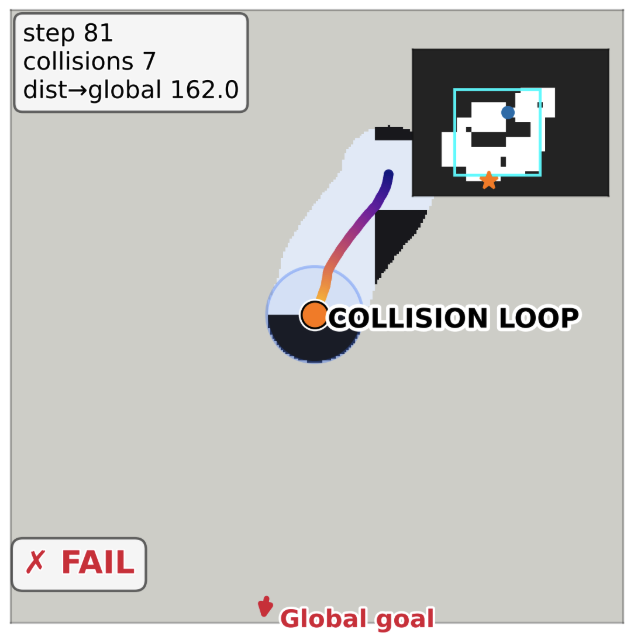
\includegraphics[width=0.29\linewidth]{baseline_D.png} \\[4pt]
  
  \rotatebox{90}{\parbox{20mm}{\centering\textcolor{green!50!black}{\textbf{Ours}}}} &
  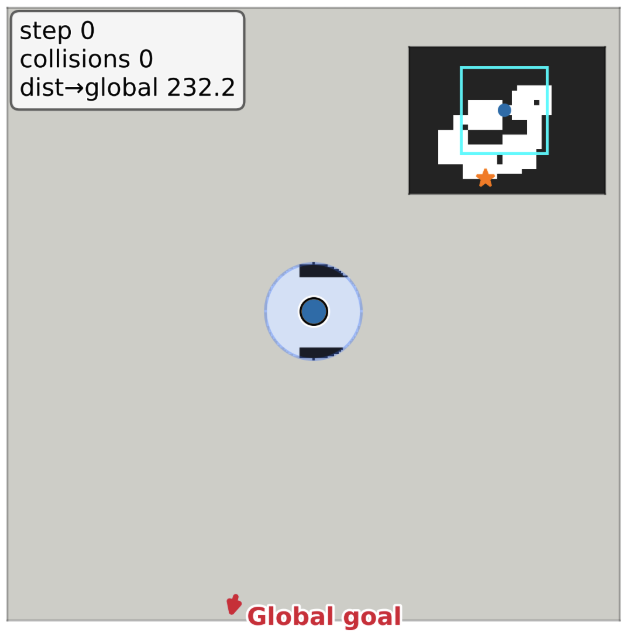
\includegraphics[width=0.29\linewidth]{ours_A.png} &
  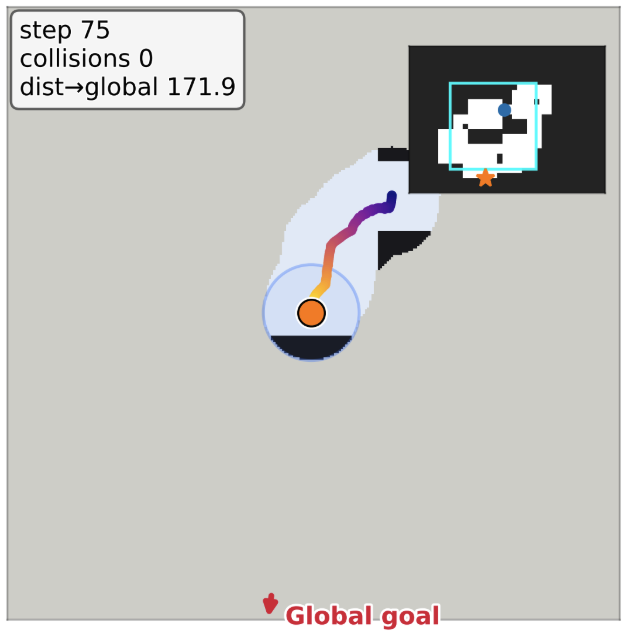
\includegraphics[width=0.29\linewidth]{ours_B.png} &
  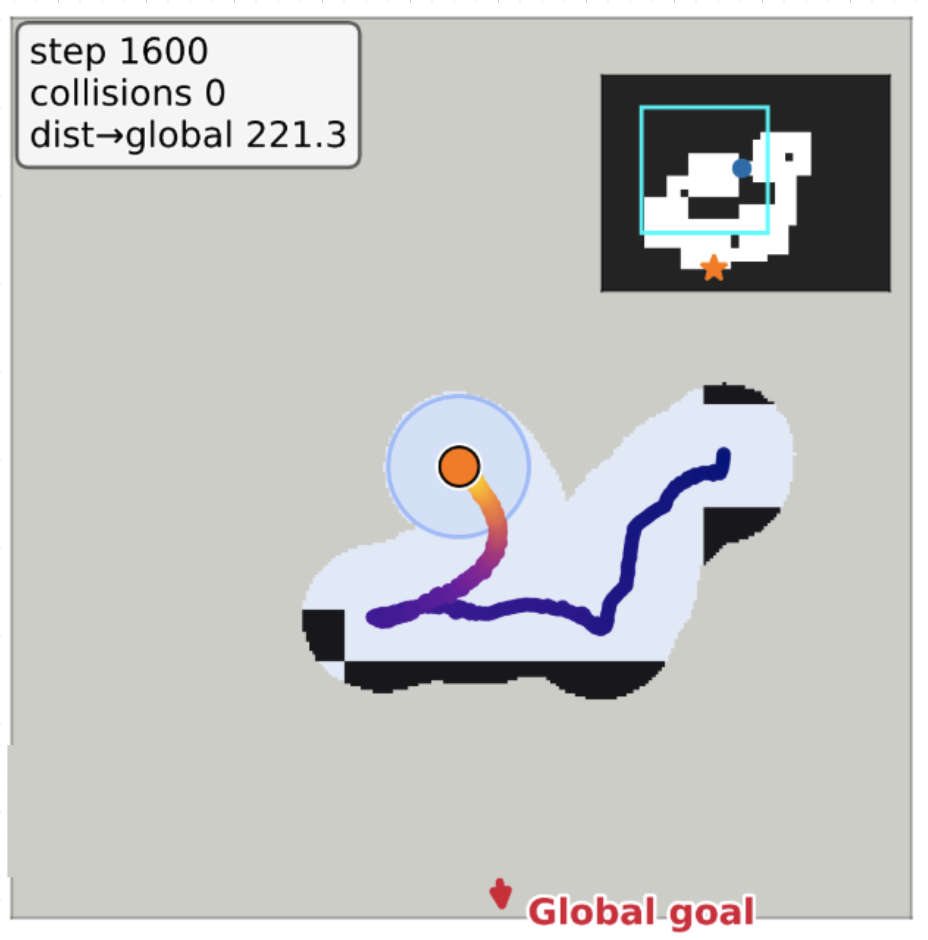
\includegraphics[width=0.29\linewidth]{ours_D.png} \\
\end{tabular}

\vspace{2mm}
{\small
\textcolor{red!65!black}{$\boldsymbol{\times}$~Frozen RL: stuck or collides}
\hfill
\textcolor{green!50!black}{$\boldsymbol{\checkmark}$~Online adaptation: reaches goal}}

\caption{\textbf{Fixed policy vs.\ online adaptation in dungeon navigation.} We display global time step, collision count, and remaining goal distance on top--left of a navigation process under a mapless environment; the inset shows the local sensed view used for decision-making. Top: a fixed RL controller executes a fixed behavior and fails by colliding / entering a collision loop as the local obstacle geometry changes.
Bottom: our method performs \emph{online correction} by adjusting its motion field using only short-horizon feedback (clearance, distance-to-goal, and speed) to avoid obstacles and keep making progress, ultimately reaching the global goal.
}

\label{fig:teaser_online_vs_rl}
\end{figure*}

These issues are magnified in SNAM. Recent systems such as Simultaneous
Goal Localization and Mapping (SGoLAM)~\citep{sgolam2021}, Cognitive Mapping and Planning (CMP)~\citep{gupta2017cognitive}, and Continual Learning of Simultaneous Localization and Mapping (CL-SLAM)~\citep{clslam2022} tightly couple mapping and policy learning, often by constructing increasingly detailed metric maps that are then consumed by learned or differentiable planners. While effective, they implicitly optimize for \emph{better maps}, not necessarily \emph{minimal, task-focused exploration}. In contrast, our objective is to \emph{reach the goal along high-quality, well-weighted paths while mapping as little of the unknown environment as possible}: as new local information is revealed, the navigator should differentially refine the path and its safety margins, rather than rebuilding global plans from scratch.

\paragraph{From unstructured policies to geometric structure.}
We view these limitations as symptoms of treating navigation as structureless optimization. Real robots are constrained by physics: conservation laws, kinematics, actuator limits, and contact constraints. Policies that ignore this structure are difficult to train, hard to interpret, and unstable over long rollouts. A geometric, physics-grounded formulation offers three advantages:
(i) \emph{Physical realizability}: dynamics remain compatible with real actuators and constraints;
(ii) \emph{Stability}: symplectic structure preserves invariants (e.g., energy, momentum) and mitigates long-horizon drift;
(iii) \emph{Compositionality}: complex behavior emerges from composing interpretable energy terms (goal attraction, collision barriers, deformation costs) that can be reweighted and adapted without relearning from scratch.

\begin{figure*}[htbp]
\centering
\begin{tikzpicture}[
  font=\small,
  panel/.style={
    draw=black!15,
    rounded corners=3pt,
    line width=0.6pt,
    inner sep=0pt,
  },
  lab/.style={
    font=\sffamily\scriptsize,
    text=white,
    fill=black!70,
    rounded corners=2pt,
    inner sep=3pt,
  },
  timestep/.style={
    font=\sffamily\scriptsize,
    text=teal!70!black,
    fill=teal!10,
    rounded corners=2pt,
    inner sep=2.5pt,
  },
  stagebadge/.style={
    font=\sffamily\small\bfseries,
    text=white,
    fill=teal!70!black,
    circle,
    minimum size=16pt,
    inner sep=0pt,
  },
  goalstyle/.style={fill=green!50!black},
  summarystyle/.style={fill=black!50},
]

\def\W{0.30\textwidth}  % Good balance
\def\H{6pt}
\def\V{8pt}

% === ROW 1 ===
\node[panel] (p1) {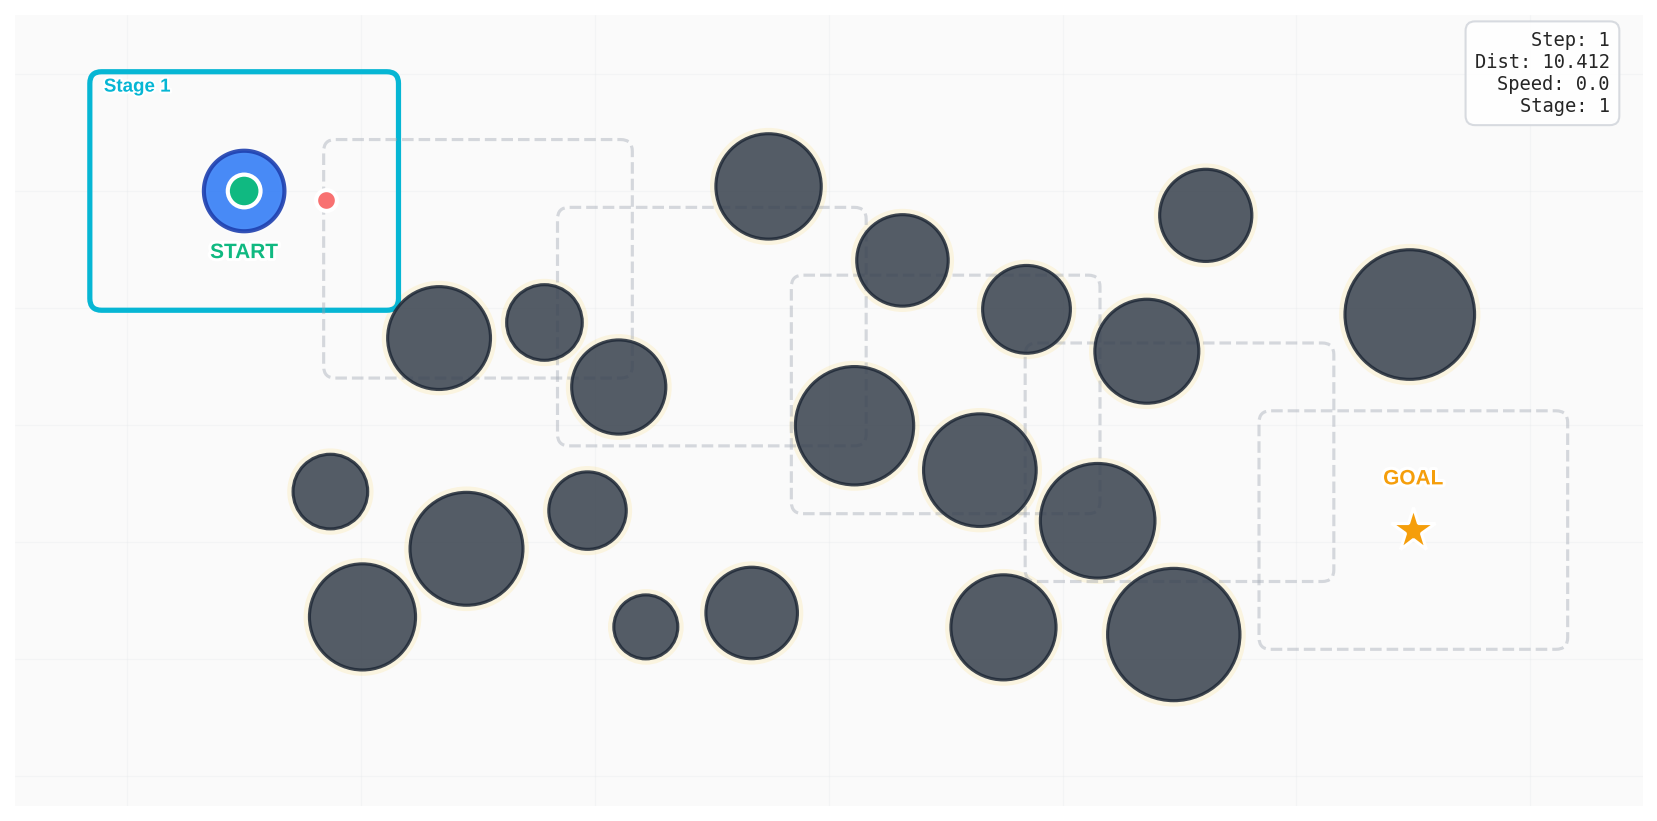
\includegraphics[width=\W]{frame_0000.png}};
\node[panel, right=\H of p1] (p2) {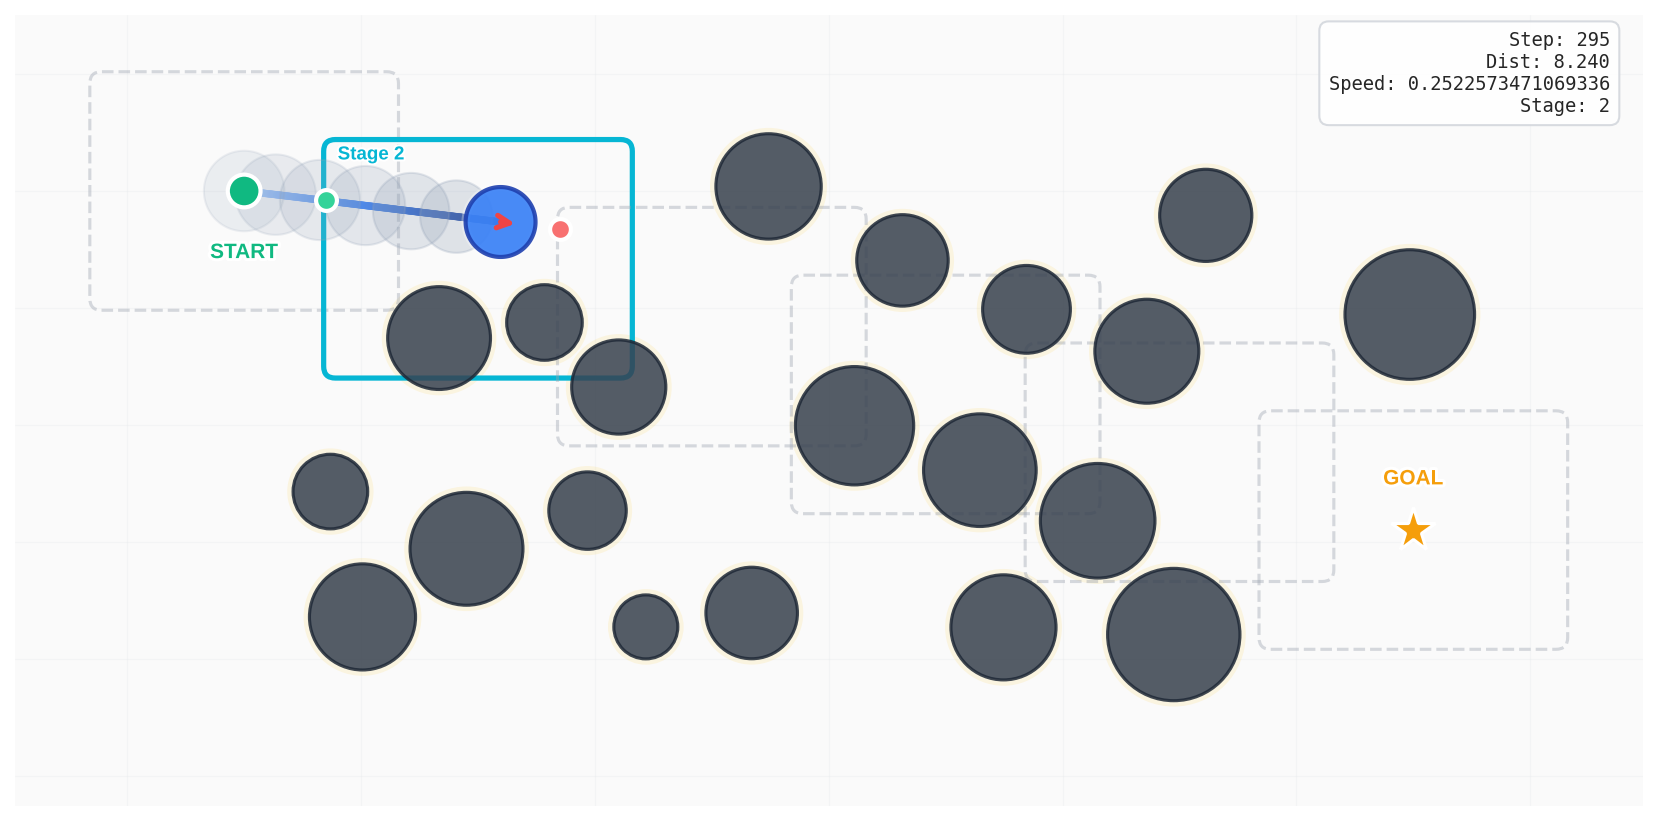
\includegraphics[width=\W]{frame_0294.png}};
\node[panel, right=\H of p2] (p3) {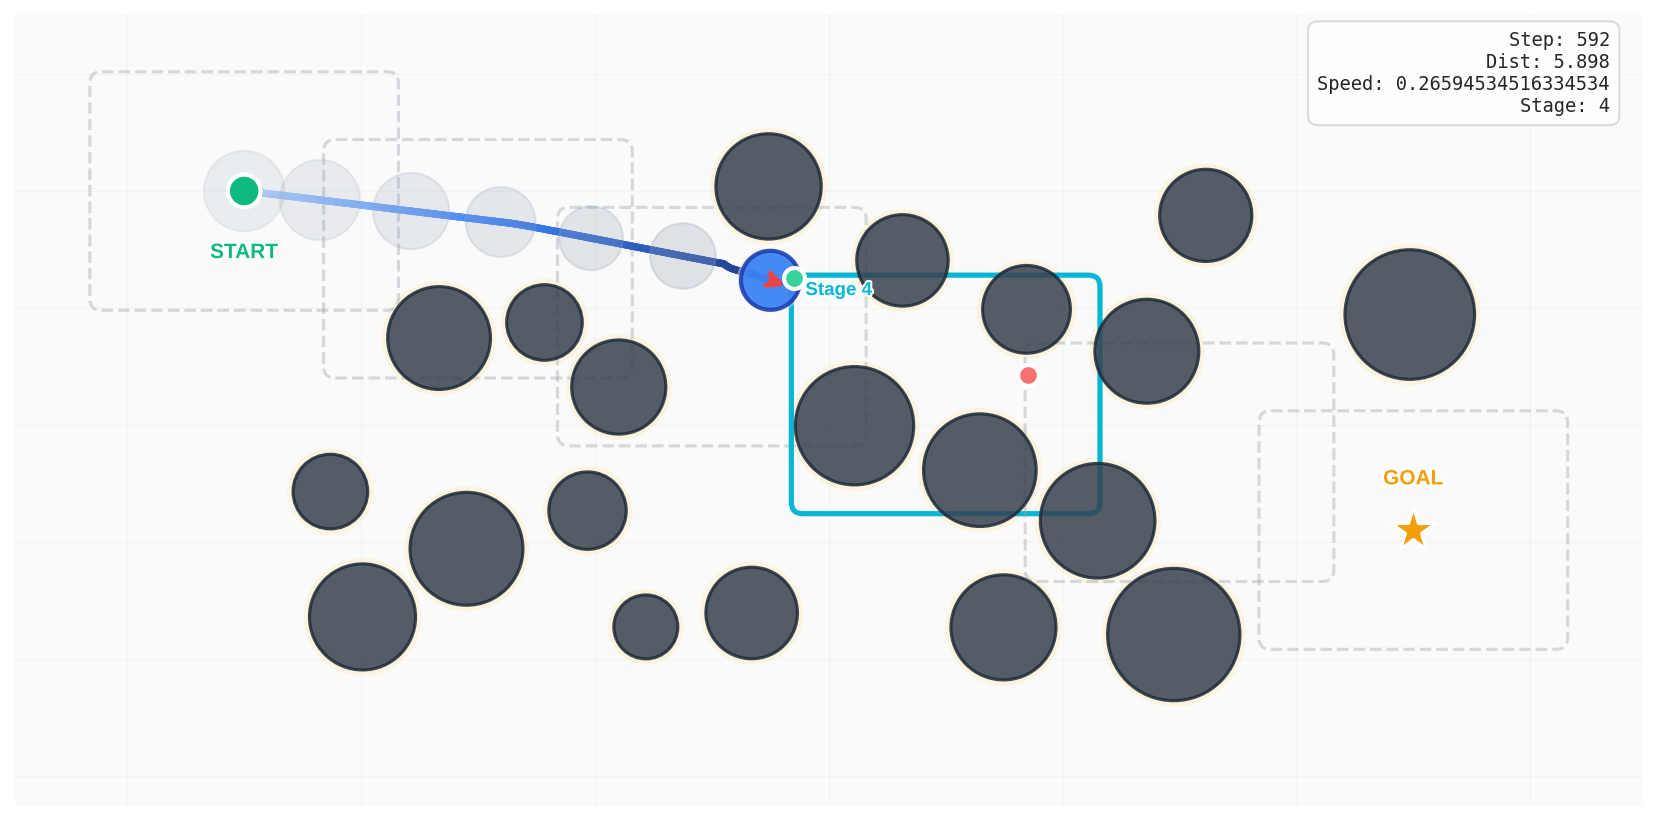
\includegraphics[width=\W]{frame_0591.png}};

% === ROW 2 ===
\node[panel, below=\V of p1] (p4) {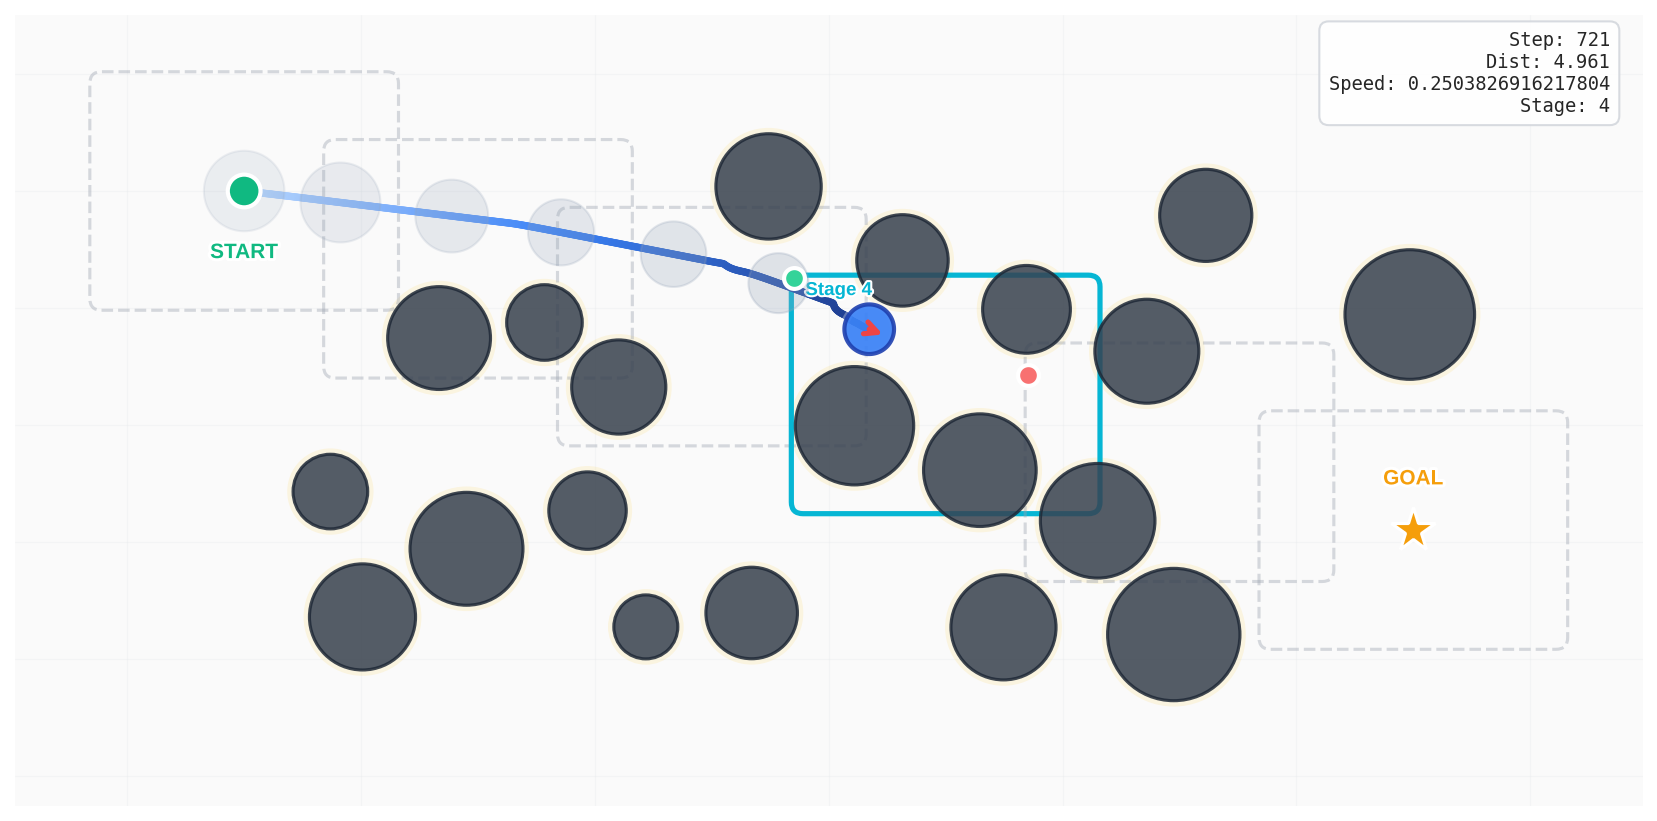
\includegraphics[width=\W]{frame_0720.png}};
\node[panel, right=\H of p4] (p5) {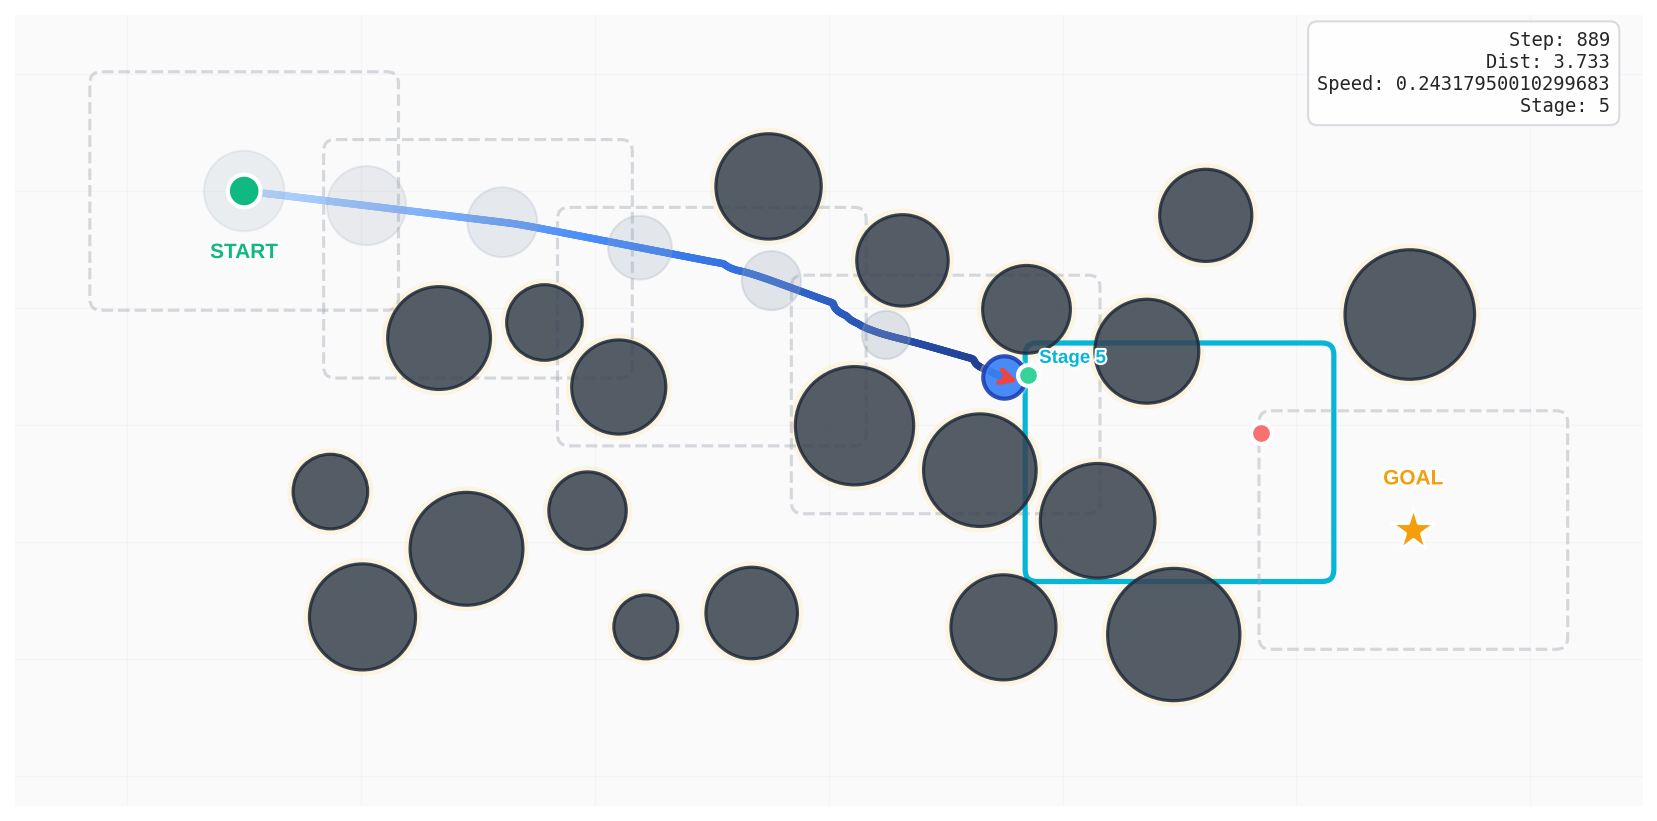
\includegraphics[width=\W]{frame_0888.png}};
\node[panel, right=\H of p5] (p6) {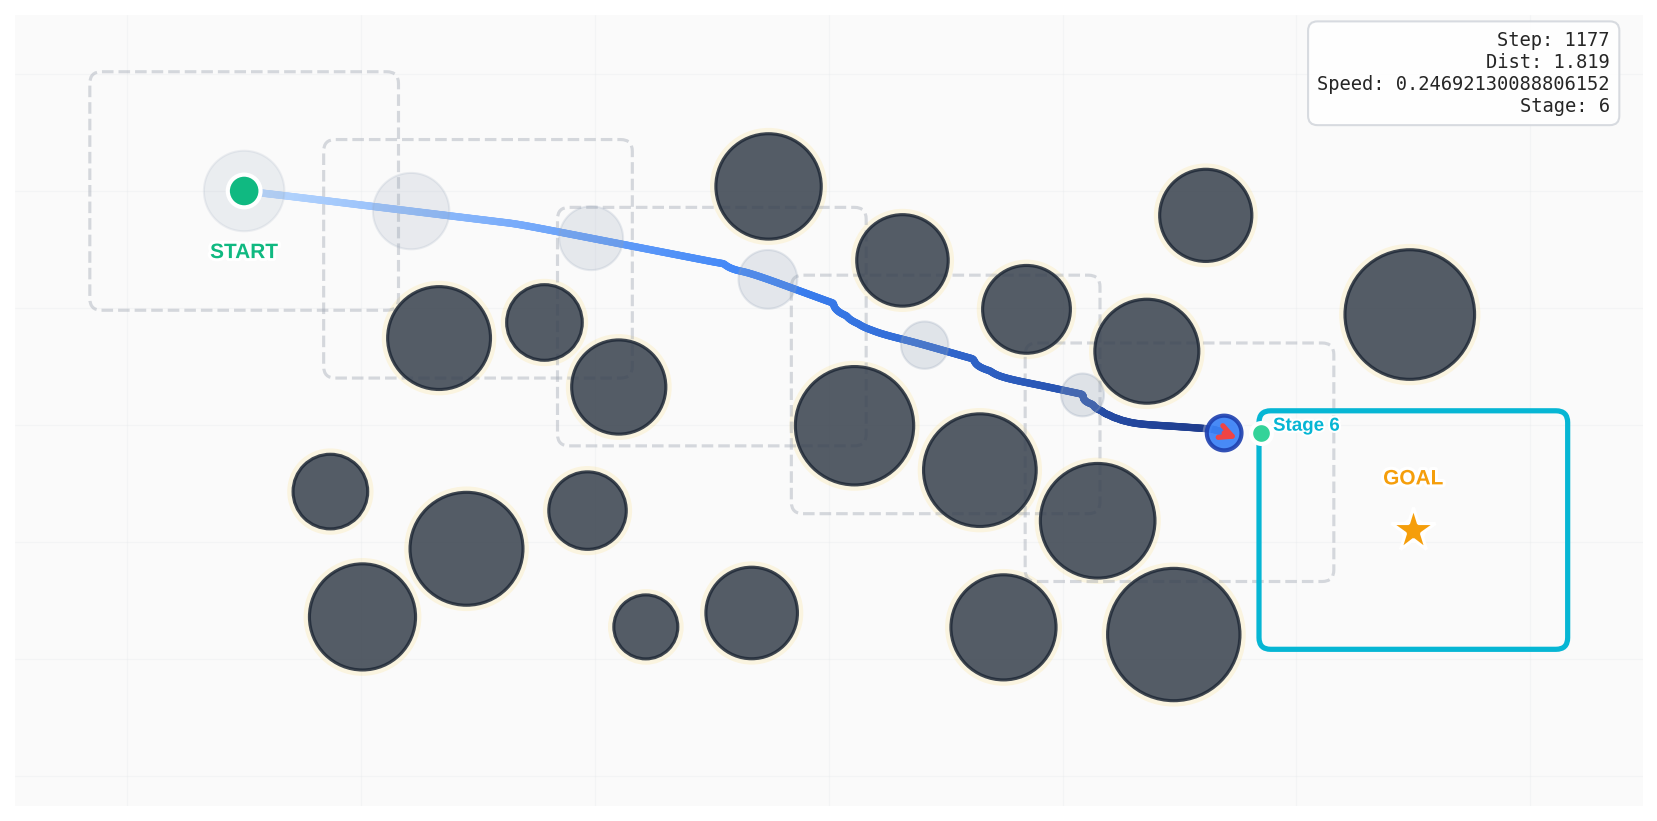
\includegraphics[width=\W]{frame_1176.png}};

% === ROW 3 ===
\node[panel, below=\V of p4] (p7) {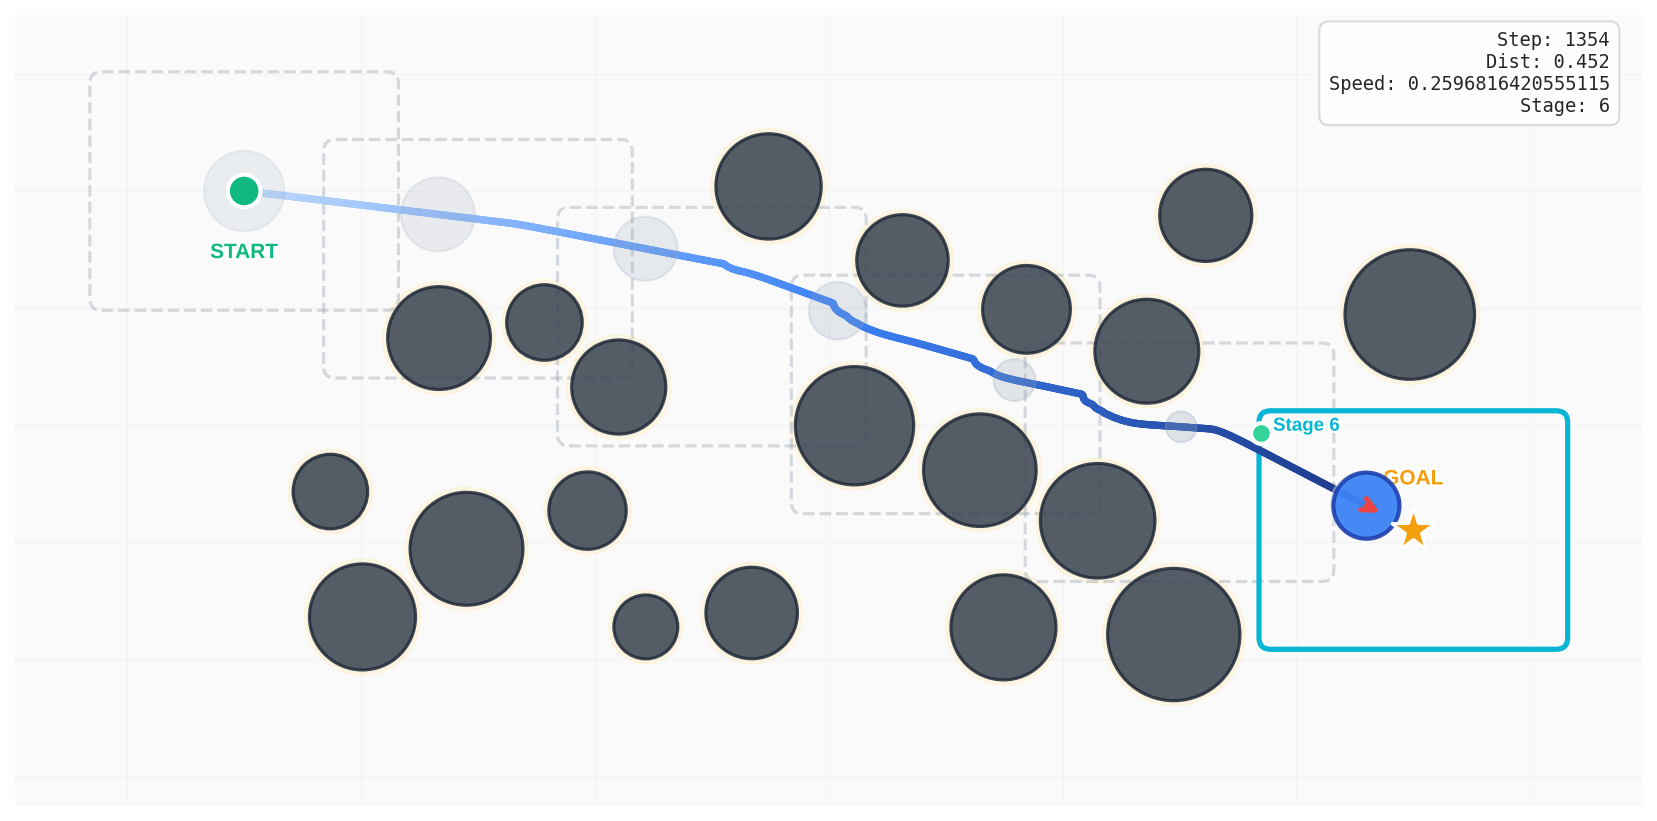
\includegraphics[width=\W]{frame_1353.png}};
\node[panel, right=\H of p7] (p8) {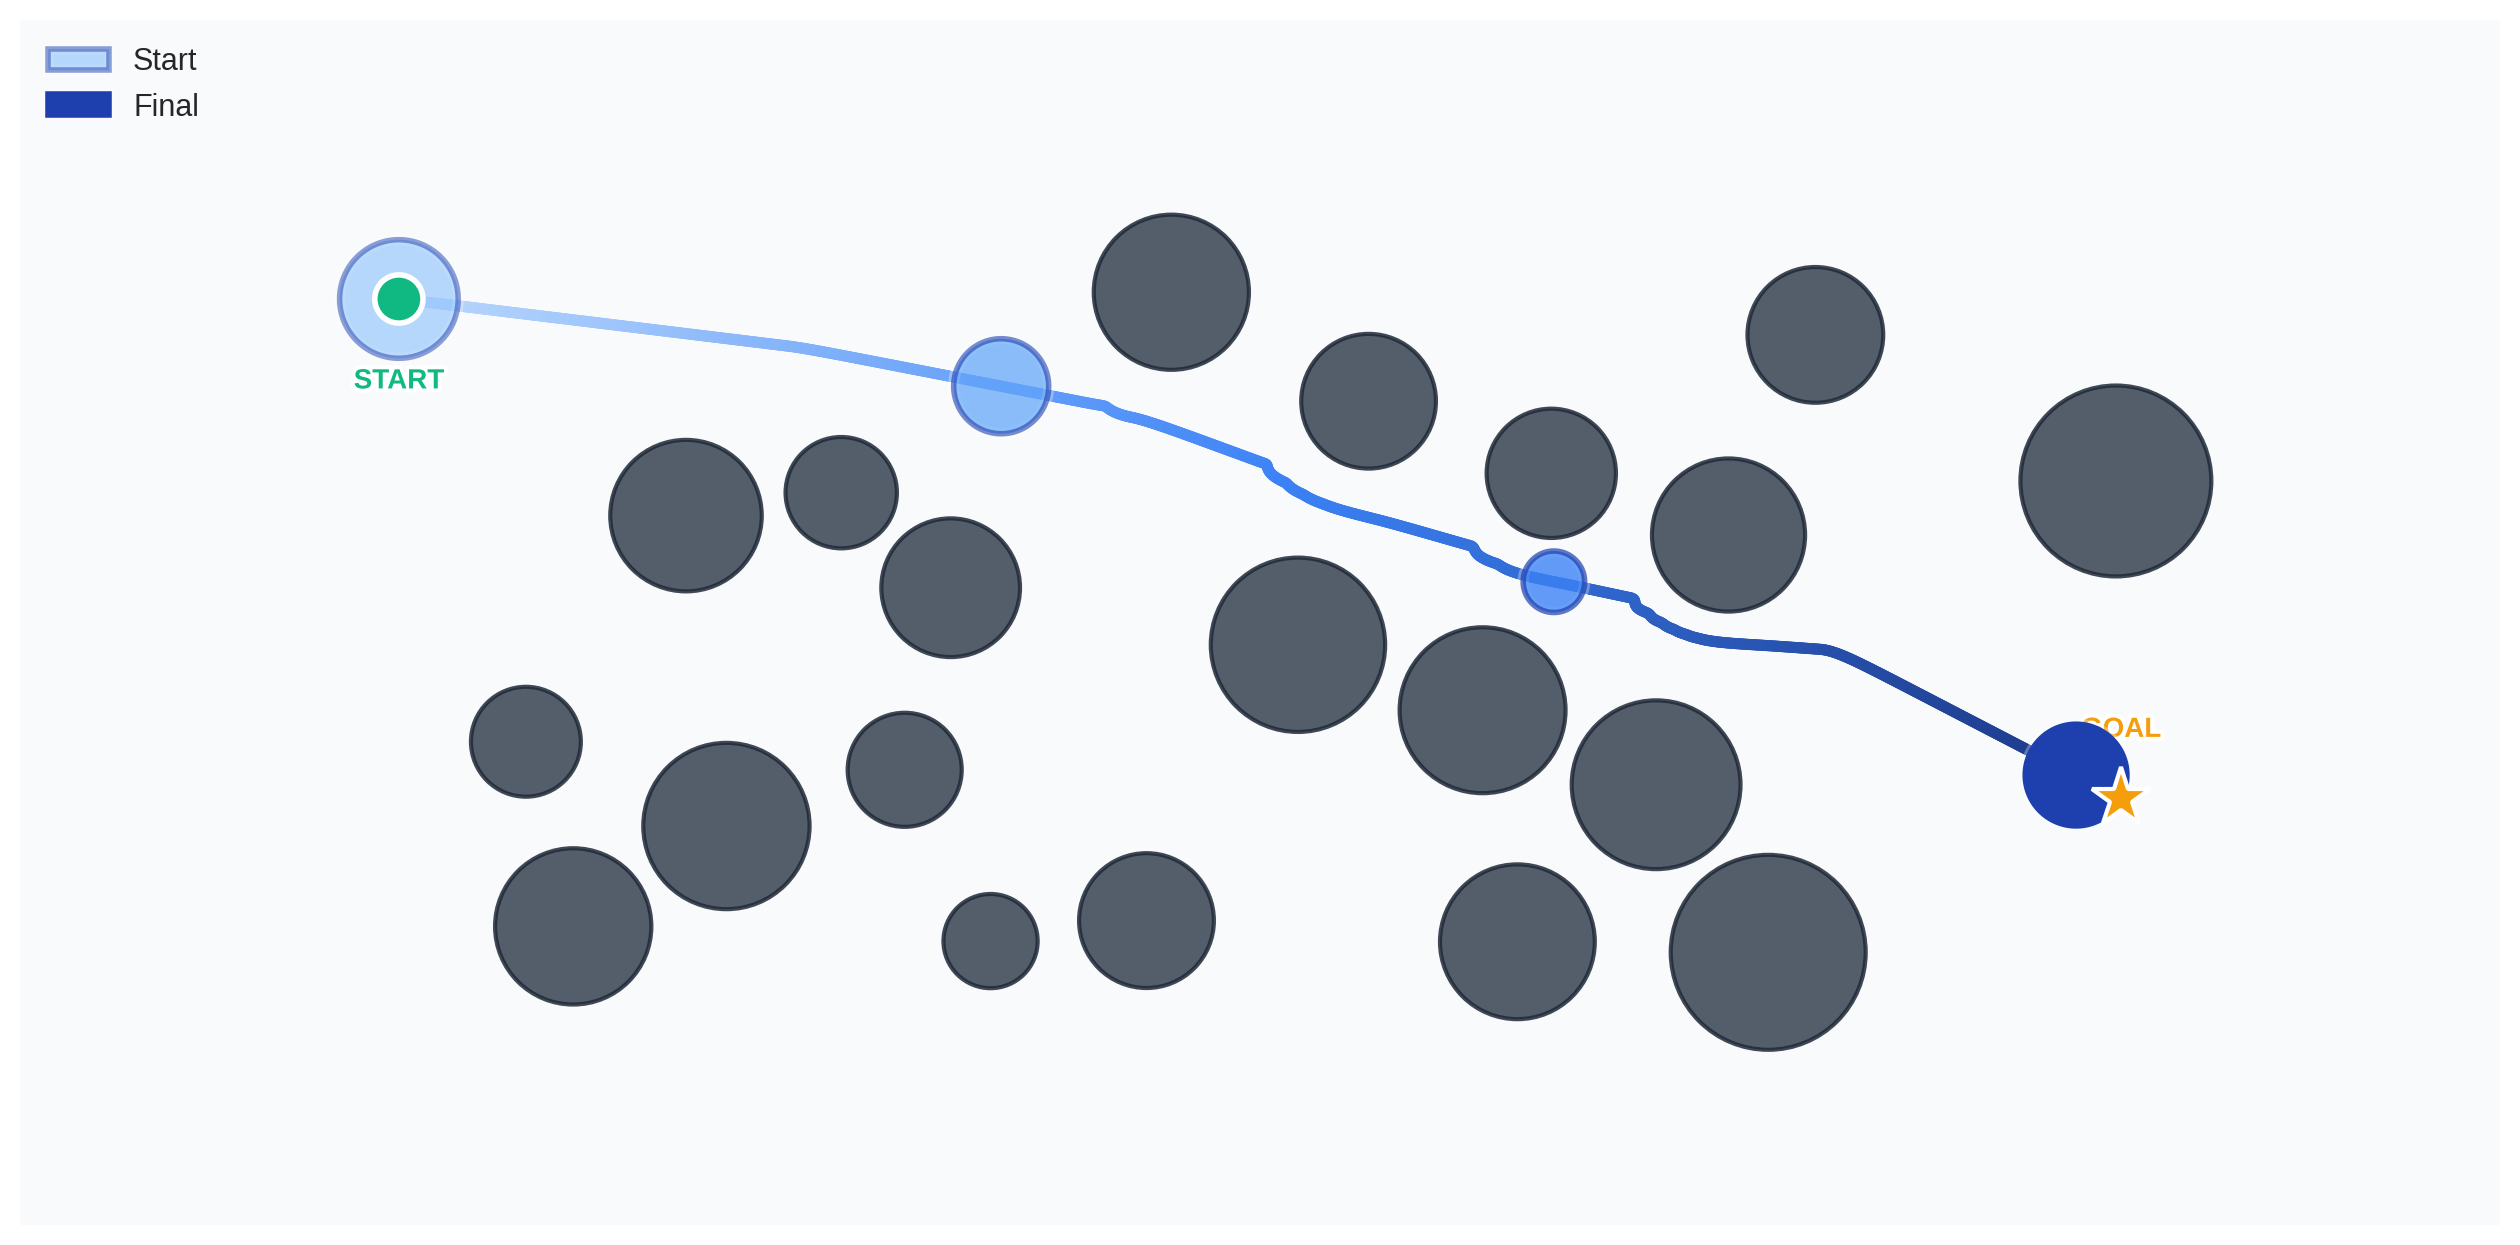
\includegraphics[width=\W]{hero.png}};
% Optional: leave third slot empty or add another view
% \node[panel, right=\H of p8] (p9) {\includegraphics[width=\W]{energy_map.png}};

% Stage badges
\node[stagebadge] at ($(p1.north east)+(-9pt,-9pt)$) {1};
\node[stagebadge] at ($(p2.north east)+(-9pt,-9pt)$) {2};
\node[stagebadge] at ($(p3.north east)+(-9pt,-9pt)$) {4};
\node[stagebadge] at ($(p4.north east)+(-9pt,-9pt)$) {4};
\node[stagebadge] at ($(p5.north east)+(-9pt,-9pt)$) {5};
\node[stagebadge] at ($(p6.north east)+(-9pt,-9pt)$) {6};
\node[stagebadge, goalstyle] at ($(p7.north east)+(-9pt,-9pt)$) {\checkmark};
\node[stagebadge, summarystyle] at ($(p8.north east)+(-9pt,-9pt)$) {$\Sigma$};

% Timesteps
\node[timestep, anchor=north west] at ($(p1.north west)+(2pt,-2pt)$) {t\,=\,1};
\node[timestep, anchor=north west] at ($(p2.north west)+(2pt,-2pt)$) {t\,=\,295};
\node[timestep, anchor=north west] at ($(p3.north west)+(2pt,-2pt)$) {t\,=\,592};
\node[timestep, anchor=north west] at ($(p4.north west)+(2pt,-2pt)$) {t\,=\,721};
\node[timestep, anchor=north west] at ($(p5.north west)+(2pt,-2pt)$) {t\,=\,889};
\node[timestep, anchor=north west] at ($(p6.north west)+(2pt,-2pt)$) {t\,=\,1177};
\node[timestep, anchor=north west] at ($(p7.north west)+(2pt,-2pt)$) {t\,=\,1354};
\node[timestep, anchor=north west, fill=black!10, text=black!50] at ($(p8.north west)+(2pt,-2pt)$) {summary};

% Labels
\node[lab, anchor=south west] at ($(p1.south west)+(2pt,2pt)$) {Initialization};
\node[lab, anchor=south west] at ($(p2.south west)+(2pt,2pt)$) {Corridor commit};
\node[lab, anchor=south west] at ($(p3.south west)+(2pt,2pt)$) {Bottleneck entry};
\node[lab, anchor=south west] at ($(p4.south west)+(2pt,2pt)$) {Squeeze-through};
\node[lab, anchor=south west] at ($(p5.south west)+(2pt,2pt)$) {Recovery};
\node[lab, anchor=south west] at ($(p6.south west)+(2pt,2pt)$) {Final approach};
\node[lab, goalstyle, anchor=south west] at ($(p7.south west)+(2pt,2pt)$) {Goal reached};
\node[lab, summarystyle, anchor=south west] at ($(p8.south west)+(2pt,2pt)$) {Full trajectory};

% Time arrows
\draw[->, >=stealth, line width=0.8pt, teal!50!black]
  ($(p1.north west)+(0,10pt)$) -- ($(p3.north east)+(0,10pt)$)
  node[midway, above, font=\sffamily\scriptsize\itshape, text=teal!60!black] {time};
\draw[->, >=stealth, line width=0.8pt, teal!50!black]
  ($(p4.north west)+(0,5pt)$) -- ($(p6.north east)+(0,5pt)$);
\draw[->, >=stealth, line width=0.8pt, teal!50!black]
  ($(p7.north west)+(0,5pt)$) -- ($(p8.north east)+(0,5pt)$);

\end{tikzpicture}
\caption{%
\textbf{GRL-SNAM rollout on a cluttered layout (representative episode).}
Snapshots are ordered left-to-right within each row, with time increasing across rows.
\emph{Row 1:} initialization ($t{=}1$) and early \emph{corridor commitment} ($t{=}295$), followed by \emph{bottleneck entry} ($t{=}592$).
\emph{Row 2:} \emph{squeeze-through} of the narrow passage ($t{=}721$), \emph{recovery/re-centering} ($t{=}889$), and \emph{final approach} to the goal ($t{=}1177$).
\emph{Row 3:} successful arrival ($t{=}1354$) and the full-trajectory overlay.
Circular stage markers
(\protect\tikz[baseline=-0.5ex]{\protect\node[font=\tiny\sffamily\bfseries, text=white, fill=teal!70!black, circle, minimum size=10pt, inner sep=0pt] {n};})
denote the active hierarchical planning stage selected by the navigator at that snapshot.%
}
\label{fig:teaser_3col}
\end{figure*}


\paragraph{GRL--SNAM: a geometric multi-policy, path-learner navigator process.} We introduce \textbf{GRL--SNAM}, a \emph{Geometric RL framework for Simultaneous Path Navigation and Mapping}, that realize SNAM policy learning via learning to formulate Hamiltonian dynamics. Our main contributions are:

\begin{enumerate}
\item \textbf{Geometric RL framework for SNAM via Hamiltonians (\cref{subsec:problem_formulation}).}
We cast navigation and mapping as formulating  control optimization problem sequentially.
The optimal control problems(OCPs) are mapped to the problem of learning the blue geometry and topology of Hamiltonian landscape through Hamiltonian dynamics. This yields our geometric RL model: it produces differentiable updates of the Hamiltonian. Differentiation in phase space corresponds to a policy update, while variation across environments induces a meta-level adaptation rule {for the lowest amortized cost to move}.


\item \textbf{Multi-scale geometric coordination via multi-policy energies (\cref{subsec:modular_architecture}).}
We introduce a three-submodular-policy architecture whose local policy govern sensing, frame-level motion, and shape control. GRL-SNAM composes each policy via constructing induced Hamiltonian flow maps and realize a discrete, feedforward Hamiltonian dynamics rather than { a backward--forward Hamiltonian-Jacobi-Bellman  optimization}. This achieves temporal scale separation without hand-designed hierarchies as well.

\item \textbf{Physics-grounded offline--online adaptation (\cref{subsec:navigator_meta_learner}).}
Building on our Geometric RL framework, we learn { Hamiltonians via a hybrid offline--online learning scheme}. During offline training, from trajectory and velocity observations, we identify the family of admissible control objectives consistent with each context and learn an embedding of the resulting landscape of local OCPs. While generalizing to unseen, online environments, our method performs online geometric alignment by adapting input-source terms naturally in Hamiltonian dynamics. This { repeated--online} adaptation strategy yields stable, low-variance adaptation that preserves { geometric, topological and functional (i.e. motion physics)} structure.

\item \textbf{Empirical validation on deformable navigation (\cref{sec:experiments}).}
On a challenging hyperelastic ring robot that must squeeze through cluttered, narrow passages, GRL--SNAM achieves higher success rates, better safety margins, and superior sample efficiency compared to { many} standard deep RL baselines (SAC, {TRPO}, PPO), as well as task-specific navigation and mapping baselines such as potential-field (PF) planners, control barrier functions (CBF), and A$^{\star}$-based methods. 
\end{enumerate}


Together, these claims support our rudiments: \textbf{when policy update respects geometric and Hamiltonian structure, complex navigation and mapping behaviors emerge naturally from energy reshaping rather than from brittle reward engineering or value iteration}. We demonstrate this principle on deformable robot navigation in unknown environments, a testbed that captures the core difficulties of real-world SNAM while showcasing the benefits of physics-informed policy design.



